\documentclass{cmspaper}
\begin{document}

%==============================================================================
% title page for few authors

\begin{titlepage}

% select one of the following and type in the proper number:
   \cmsnote{2008/000}
%  \internalnote{2005/000}
%  \conferencereport{2005/000}
   \date{23 July 2008}

  \title{Photon Identification for CMS Startup}

  \begin{Authlist}
    A.~Askew, O.~Atramentov, Y.~Gershtein,
       \Instfoot{FSU}{Florida State University, Tallahassee, FL.}

    A.~Debenedetti,
	\Instfoot{Minn}{University of Minnesota, Minneapolis, MN.}

    M.~Gataullin, V.~Litvin, J.~Veverka, 
	\Instfoot{CalTech}{California Institute of Technology, Pasadena, CA.}

    T.~Miceli, J.~Stilley,
	\Instfoot{UCDavis}{University of California at Davis, Davis, CA.}

    V.~Gaultney,
        \Instfoot{FIU}{Florida International University, Miami, FL.}

    S.~Shrestha,
        \Instfoot{KSU}{Kansas State University, Manhattan, KS.}

    M.~Anderson,
        \Instfoot{Wisc}{University of Wisconsin, Madison, WI.}

    J.~Lamb
        \Instfoot{UCSB}{University of California at Santa Barbara, Santa Barbara, CA.}

  \end{Authlist}

% if needed, use the following:
%\collaboration{Flying Saucers Investigation Group}
%\collaboration{CMS collaboration}

  \begin{abstract}
This note defines the methods by which the identification of photons may be verified from data
on start up.  This verification includes measurement of the photon efficiency, as well as methods
for obtaining photon purity.  Backgrounds to photons from jets and electrons are discussed, and an
example set of ``vanilla'' photon identification requirements are presented. 
  \end{abstract} 

% if needed, use the following:
%\conference{Presented at {\it Physics Rumours}, Coconut Island, April 1, 2005}
%\submitted{Submitted to {\it Physics Rumours}}
%\note{Preliminary version}
  
\end{titlepage}
\tableofcontents
\listoffigures
\listoftables
\pagebreak

\setcounter{page}{2}%JPP

\section{Introduction}
Photon identification at hadron colliders is a difficult task, mainly due to the large backgrounds from hadronic jets and
the lack of a clean large cross-section resonance decaying into high $E_T$ photons for studies.  
Radiative decays $Z\gamma\rightarrow\ell\ell\gamma$ events in which the photon is radiated off one of the final state leptons 
can be selected and used for photon calibration \cite{uug_note}, but the rate of this decay is small and photons tend to be soft.
This difficulty is further compounded by the fact that unlike electrons,
photons are not redundant
\footnote{Unconverted photons are not redundant.  For the special case of conversions with reconstructed
tracks, please see~\cite{NancyConv}.}, e.g. they leave a signal in only one detector, the electromagnetic calorimeter.  
Thus, unlike electrons, tracker and calorimeter information can not be compared to get a handle on the reconstruction efficiency.
Also, photons are subject to backgrounds (such as cosmic/halo muon bremsstrahlung) which do not typically afflict electrons.
Special techniques are being developed to measure and reduce these non-collision backgrounds.

This note describes a possible strategy for doing physics with photons at very early stages of the experiment.
CMS detector combines very heavy tracker with very strong magnetic field. The effects of both on electrons and photons are very significant, and are 
unlikely to be well-described by the Monte Carlo simulation in the beginning of the run. 
We show that a moderately effective photon identification can be constructed so that its efficiency and purity can be reliably measured with
data itself.

We show that some identification variables, like hollow cone track isolation and cluster width in $\eta$, are quite similar between electrons and 
photons and therefore can be calibrated using $Z \rightarrow e e$ decays. 
These efficiencies can then be (to the limit of available statistics) verified with early samples of $Z\gamma\rightarrow\ell\ell\gamma$.  
We also show that selecting photon candidates failing hollow cone track isolation in multi-jet events 
provides us with a clean sample of pure and minimally biased jet background for fake rate determination.


\section{Photon Reconstruction and LooseEM}

In order to utilize the flexibility of the photon reconstruction software, a base definition {\bf LooseEM} is defined to provide a starting point for both signal and background studies\footnote{There is a software delineation between the EgammaPhotonProducer package, which constructs the actual reco::Photon, and the PhotonIdentification package which is mainly concerned with the organization and analysis of reco::Photon objects.  The interested reader is referred to Appendix B.}.  The object of the {\bf LooseEM} definition is to provide a definition of objects that are reconstructed as photons which are 100\% efficient for true photons (produced in collisions), but provides some rejection against fake photons from hadronic activity. In particular, it ensures that a jet gives rise to not more than one of such objects, and that its energy is comparable to the parent parton. 

A {\bf LooseEM} for the purposes of this documents is defined as a reco::Photon which meets the following criteria:
\begin{list}{$\bullet$}
 \item{The reco::Photon must be isolated from other deposits of energy in the ECAL.  The sum of the energy deposited in a cone
of $\Delta R <$0.4 minus the energy that is clustered into the photon must be smaller than 20~GeV.  The distribution of the sum is presented in 
Figure~\ref{fig:EMiso_EMLoose}. All crystals with $E_{crys} >$ 0 GeV are considered. Higher threshold is likely to improve the discrimination
and is being optimized (also in context of electron and muon isolation).}
 \item{The reco::Photon must be isolated from surrounding deposits of energy in the HCAL.  The sum of the energy in the HCAL in
a hollow cone of 0.1 $< \Delta R<$0.4 is required to be smaller than 10~GeV.  No threshold save that the cells are above 0 GeV is applied.  
Note that the selection of this hollow cone is to make the measurement of this isolation quantity independent of the calculation of the 
hadronic-electromagnetic energy ratio which is more sensitive to EM shower leakage.}
 \item{The reco::Photon is required to have its $HadOverEM$ ratio be smaller than 0.2.  $HadOverEM$ here is defined as the energy within $\Delta R=$0.1 of the supercluster centroid in the hadronic calorimeter divided by the energy of the supercluster.}  
\end{list}

Distributions of each of these quantities are shown for nominal samples of signal and background in Figures~\ref{fig:EMiso_EMLoose},~\ref{fig:HCALiso_EMLoose}, and~\ref{fig:HadOverEM_EMLoose}.  All of these distributions are shown for barrel photons only.

\begin{figure}[hbtp]
  \begin{center}
    \resizebox{10cm}{10cm}{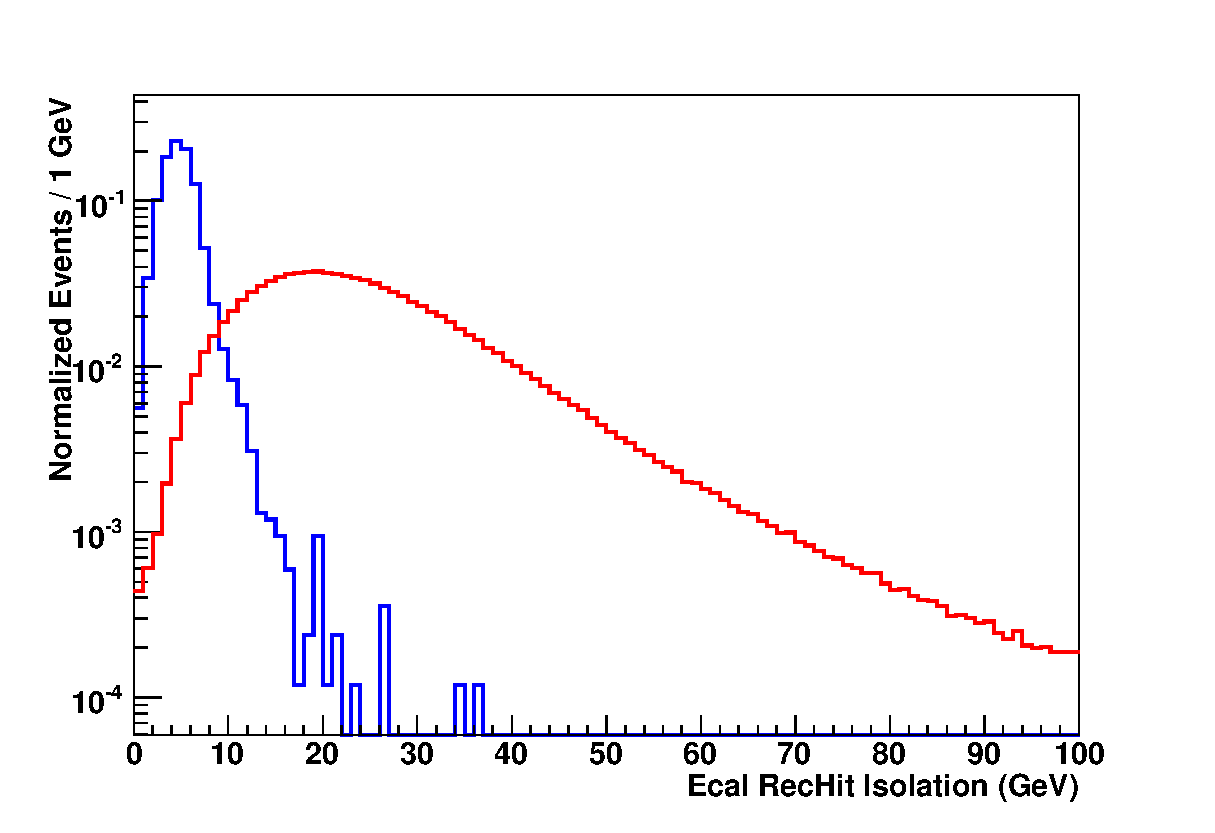
\includegraphics{EMLoose/EMiso_EMLoose.eps}}
    \caption{ECAL isolation energy for direct photons (blue) and for fakes from dijets (red).}
    \label{fig:EMiso_EMLoose}
  \end{center}
\end{figure}
\begin{figure}[hbtp]
  \begin{center}
    \resizebox{10cm}{10cm}{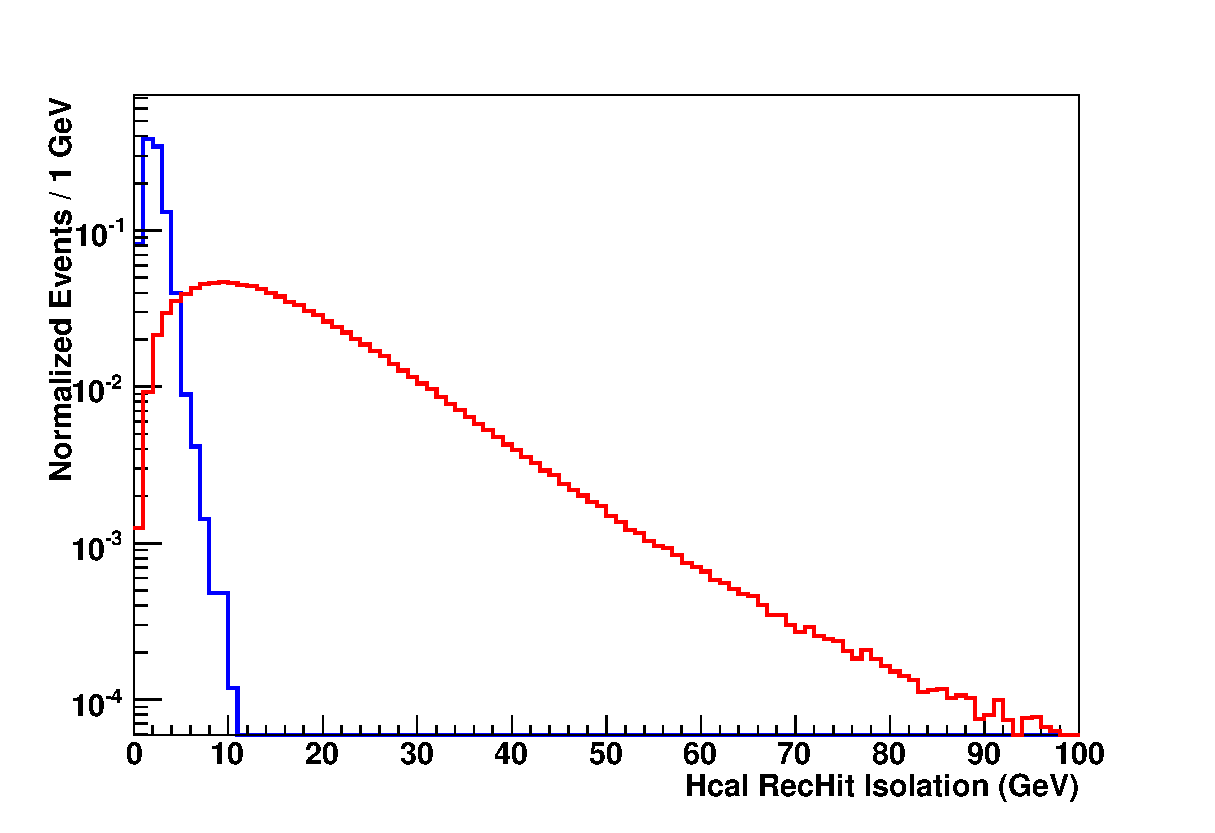
\includegraphics{EMLoose/HCALiso_EMLoose.eps}}
    \caption{HCAL isolation energy for direct photons (blue) and for fakes from dijets (red).}
    \label{fig:HCALiso_EMLoose}
  \end{center}
\end{figure}
\begin{figure}[hbtp]
  \begin{center}
    \resizebox{10cm}{10cm}{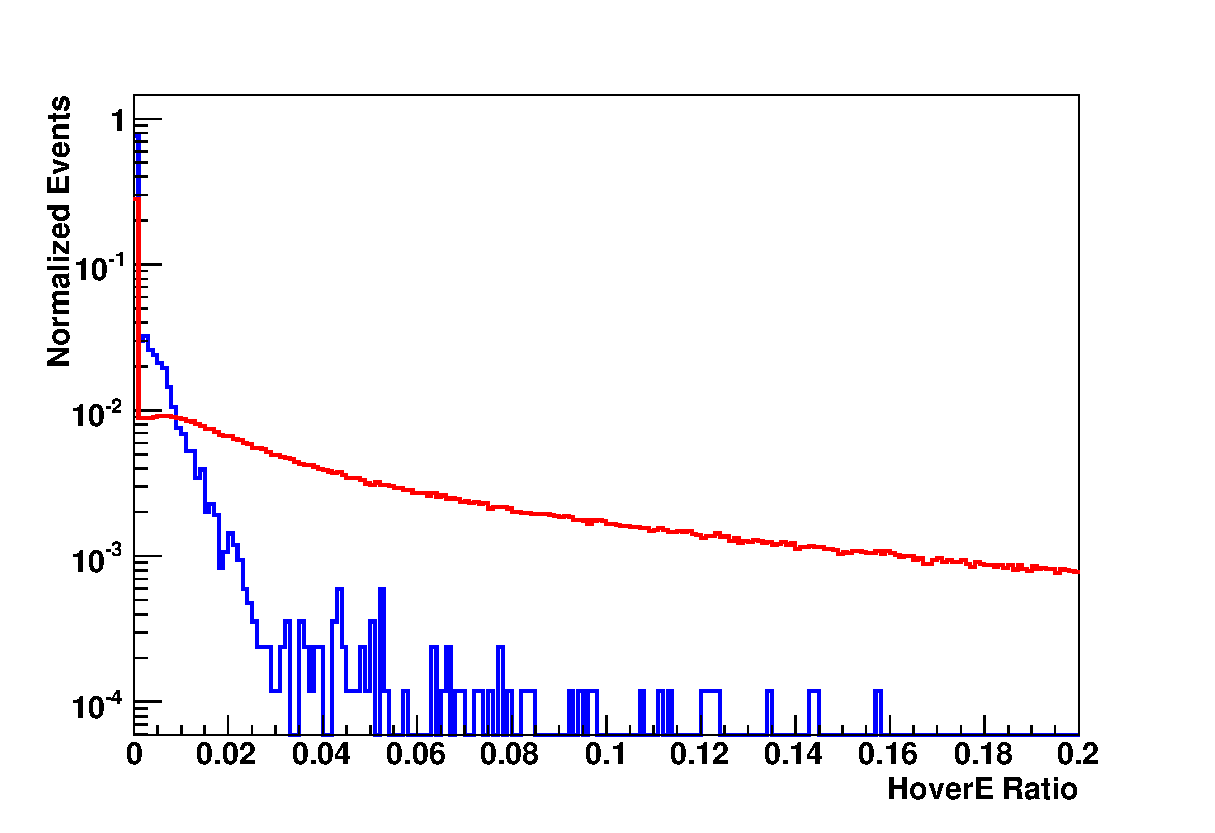
\includegraphics{EMLoose/HadOverEM_EMLoose.eps}}
    \caption{HadOverEM ratio for direct photons (blue) and for fakes from dijets (red).  No photon overflows are present.}
    \label{fig:HadOverEM_EMLoose}
  \end{center}
\end{figure}

The signal sample shown here is a sample of QCD direct photon production produced privately in CMSSW\_2\_1\_0\_pre5, in which the generated photon was required to match to a reconstructed reco::Photon object.  The background sample was a sample of inclusive QCD dijets which were produced in the official CSA08 production, which made use of CMSSW\_2\_0\_5.  As previously mentioned, only barrel photons are considered here, and further, the photon $E_{T}$ is required to be greater than 20~GeV.
As one can see, these cuts remove a significant portion of the jet background, while retaining most if not all of the true photons.  The efficiency of these cuts, and their measurement from the data is discussed in Section~\ref{ssec:LooseEMEff}.

\section{Photon Identification Quantities and Selection}
With the base {\bf LooseEM} definition in place, more specific selection cuts for photon identification may be chosen.  Two additional definitions are made here {\bf LoosePhoton} and {\bf TightPhoton}.  
A {\bf LoosePhoton} is defined as a {\bf LooseEM} with:
\begin{list}{$\bullet$}
 \item{$HadOverEM$ ratio of smaller than 0.1.}
\item{Isolation from electromagnetic activity (as defined in {\bf LooseEM}) smaller than 15 GeV.}
\item{The sum of the $p_{T}$ of tracks within a hollow cone of $\Delta R<$(0.4-0.0X) is required to be smaller than 5 GeV.}
\end{list}
A {\bf TightPhoton} satisfies all of the cuts from the {\bf LoosePhoton}, but with the additional requirement that its R9 variable (defined in Eqn.~\ref{eqn:R9}) is greater than 0.8.
\begin{equation}
 R9 = \frac{E_{3x3}}{E_{supercluster}}
\end{equation}\label{eqn:R9}
\begin{figure}[hbtp]
  \begin{center}
    \resizebox{10cm}{10cm}{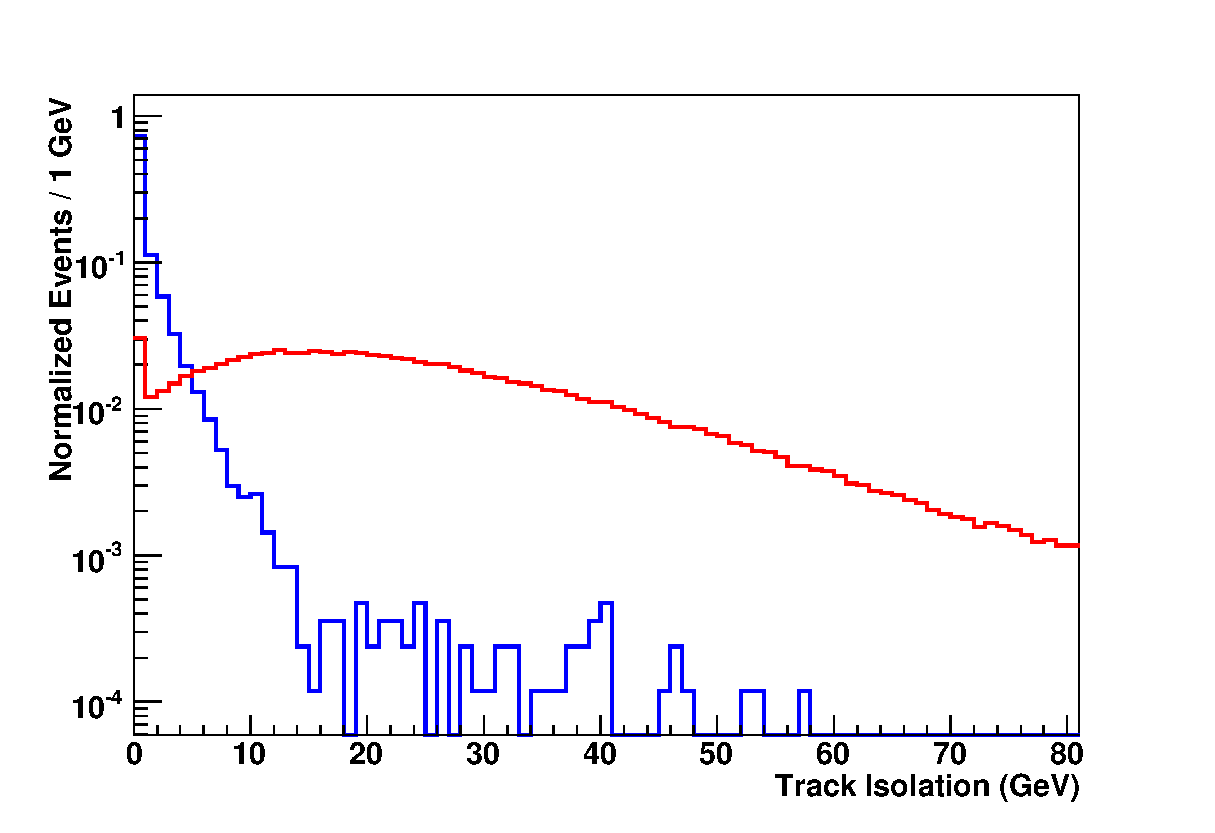
\includegraphics{PhotonSel/Photonid_trkiso.eps}}
    \caption{Sum of track $p_T$ as defined in {\bf LoosePhoton} for {\bf LooseEM} objects in direct photon events (blue) and fakes
from dijets(red).}
    \label{fig:Photonid_trkiso}
  \end{center}
\end{figure}
\begin{figure}[hbtp]
  \begin{center}
    \resizebox{10cm}{10cm}{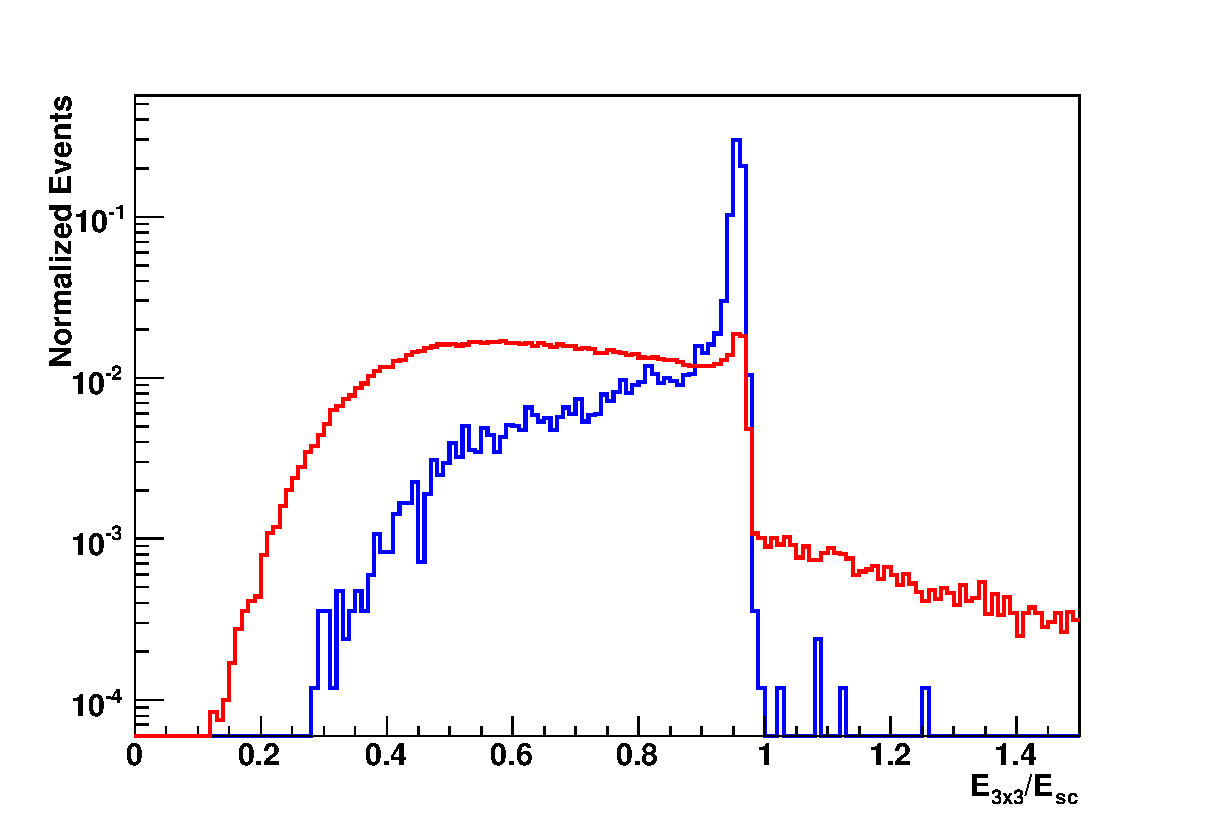
\includegraphics{PhotonSel/Photonid_r9.eps}}
    \caption{R9 variable for {\bf LooseEM} objects in direct photon events (blue) and for fakes from dijets (red).}
    \label{fig:Photonid_r9}
  \end{center}
\end{figure}

\section{Efficiency Determination in the Data}
Since photons are not redundant objects (as previously stated), the determination of the data efficiency for photon reconstruction requires more steps than the simple tag-and-probe method for electrons from $Z\rightarrow ee$ events.
The base prescription for measuring photon efficiencies in data shall be:
\begin{list}{$\bullet$}
\item{Make selection on quantities that will be as similar as possible between electrons and photons.  A good example of this is the hollow cone of the track isolation, which will be set such that for electrons the associated track will be outside this
cone such that the track isolation efficiency can be measured with electrons.}
\item{Ascertain the extent to which a cut can be made on these similar quantities.  If a cut on, say track isolation, is noticeably different between electrons and photons in the Monte Carlo, then this difference must be assigned as a systematic uncertainty.}
\item{Measure the efficiency for the given selection cuts in data using a tag-and-probe method.  Use this same tag-and-probe method to measure the efficiency in Monte Carlo, and compare with the Monte Carlo truth efficiency to check for bias.} 
\item{Scale the Monte Carlo efficiency (if necessary) to the data and calculate the final systematic uncertainty.}
\end{list}

This prescription limits one, for early data taking, to quantities that can be verified in the data from electrons.  Of course, constructing quantities that are similar for photons and electrons allows one to factorize the background somewhat, first there will be hadronic jets (which are discriminated against by the different isolation requirements), and isolated electromagnetic objects.  These electromagnetic objects, by means of a track veto, can then be separated into electrons and photons.

\subsection{LooseEM efficiency}\label{ssec:LooseEMEff}

It is very hard to measure clustering efficiency of an unconverted photon. For this, we have to rely on Monte Carlo.
However, the MC here can be cross-checked using electrons, and if the efficiency is large then the resulting systematic error can be made small. 

The {\bf LooseEM} efficiency for electrons is determined using a tag-and-probe method.  $Z$-boson events are selected first by requiring two high $p_T$ tracks, one of which is required to pass tight quality requirements and match well in $\eta-\phi$ with an electromagnetic object in the ECAL.  The second serves as a probe, and along with the cluster matched to the tag, the invariant mass can be formed, to control possible backgrounds.  The efficiency then, is the rate at which the probe track is associated with a {\bf LooseEM} object in the calorimeter.

\section{Photon Fake Rates and Purity}
\subsection{Photon-Jet Fake Rate}
\subsection{Photon-Electron Fake Rate}


\section{Additional Backgrounds to Photons}
As previously mentioned, since photons only manifest themselves as isolated clusters of energy in the electromagnetic calorimeter, they are subject to backgrounds from cosmic ray and beam halo muons which undergo bremsstrahlung in the calorimeter as they pass through.  For each of these backgrounds, one attempts to derive the contamination from these sources by identifying variables that are sensitive to the difference between these bremsstrahlung backgrounds and building templates from the data using tags.  Then along with templates from prompt electromagnetic objects in data, one can do fits to the final candidate distributions in the data to determine the final prompt fraction.

The handles that we consider are:
\begin{itemize}
\item reconstructed time in the ECAL
\item shape of the ECAL energy deposition
\item reconstructing matching (in space and time) signals in HCAL and Muon systems   
\end{itemize}

\subsection{Beam Halo Muons}

%original text from Tia, edited by A.A.
"Halo muons" are a muons that travel along with the proton beams. They are
produced by beam protons hitting residual gas (or the sides of the
beam pipe), then showering to pions, which subsequent decay to muons.
These muons could leave evidence in the CMS detector through interacting with
the material.

There is halo shielding prior to the CMS detector, and there are halo
triggers to reject halo events (or select them for the purposes of alignment). 
Some muons may still leave evidence in the recorded events.  If a muon crosses through the 
ECAL and bremsstrahlungs, this process could be mistaken for a prompt photon. 
We are currently investigating the shower shape and timing of a halo muon bremsstrahlung compared with
the shower shape and timing of prompt photons.  It is expected that halo muon
bremsstrahlung shower shape will be extended in eta (halo muons travel
parallel to beam), while the prompt photon shower shape will be well constrained, if perhaps
extended in phi (if the photon converts to an e- e+ pair, the strong
magnetic field will bend the pair to extend its energy deposit in phi).
\subsubsection{ECAL timing}

\subsubsection{shower shape}

\subsubsection{ECAL-CSC correlations}

\subsubsection{ECAL-HE correlations}


\subsection{Cosmic Ray Muons}

\subsubsection{shower shape}

\begin{figure}[hbtp]
  \begin{center}
    \resizebox{10cm}{10cm}{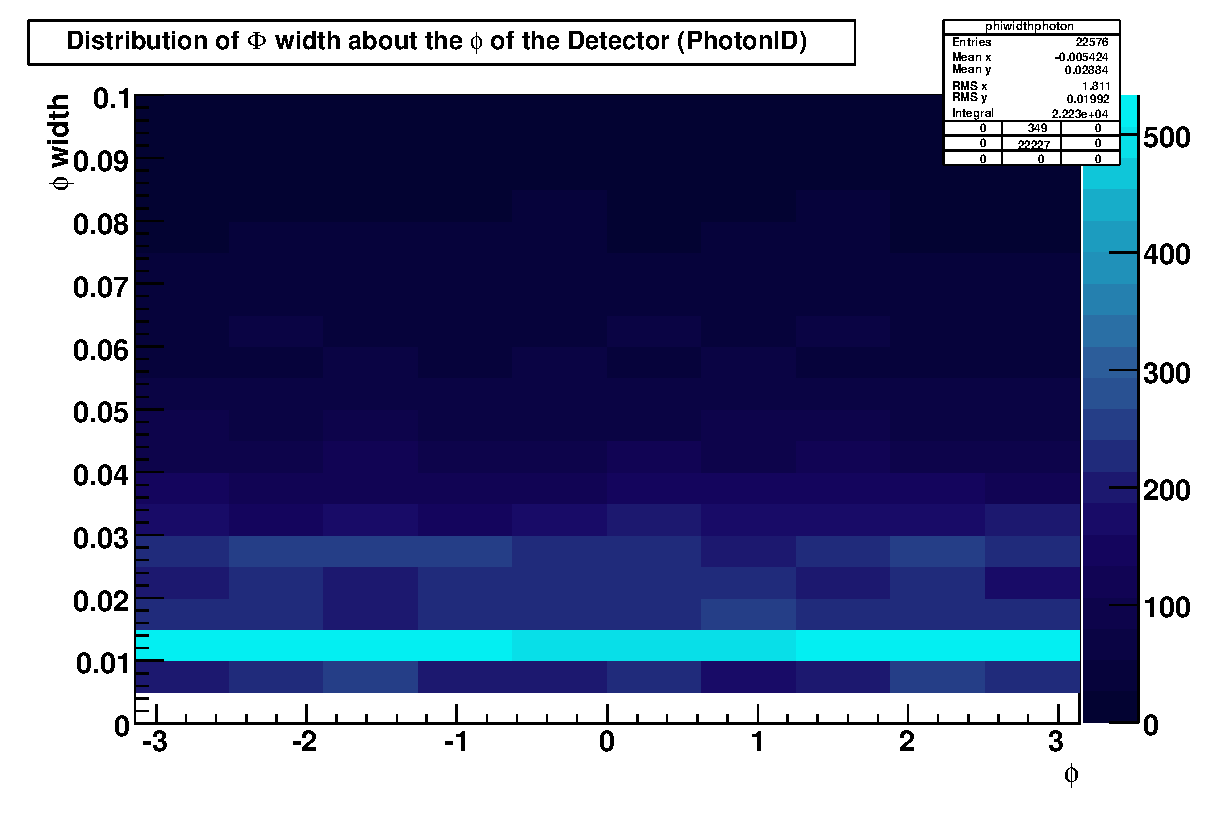
\includegraphics{CosmicPlots/photonID.eps}}
    \caption{The energy weighted width in $\phi$ as a function of detector $\phi$ for prompt, direct photons from the interaction region.  No dependence is observed.}
    \label{fig:PromptPhiWidPhi}
  \end{center}
\end{figure}

\begin{figure}[hbtp]
  \begin{center}
    \resizebox{10cm}{10cm}{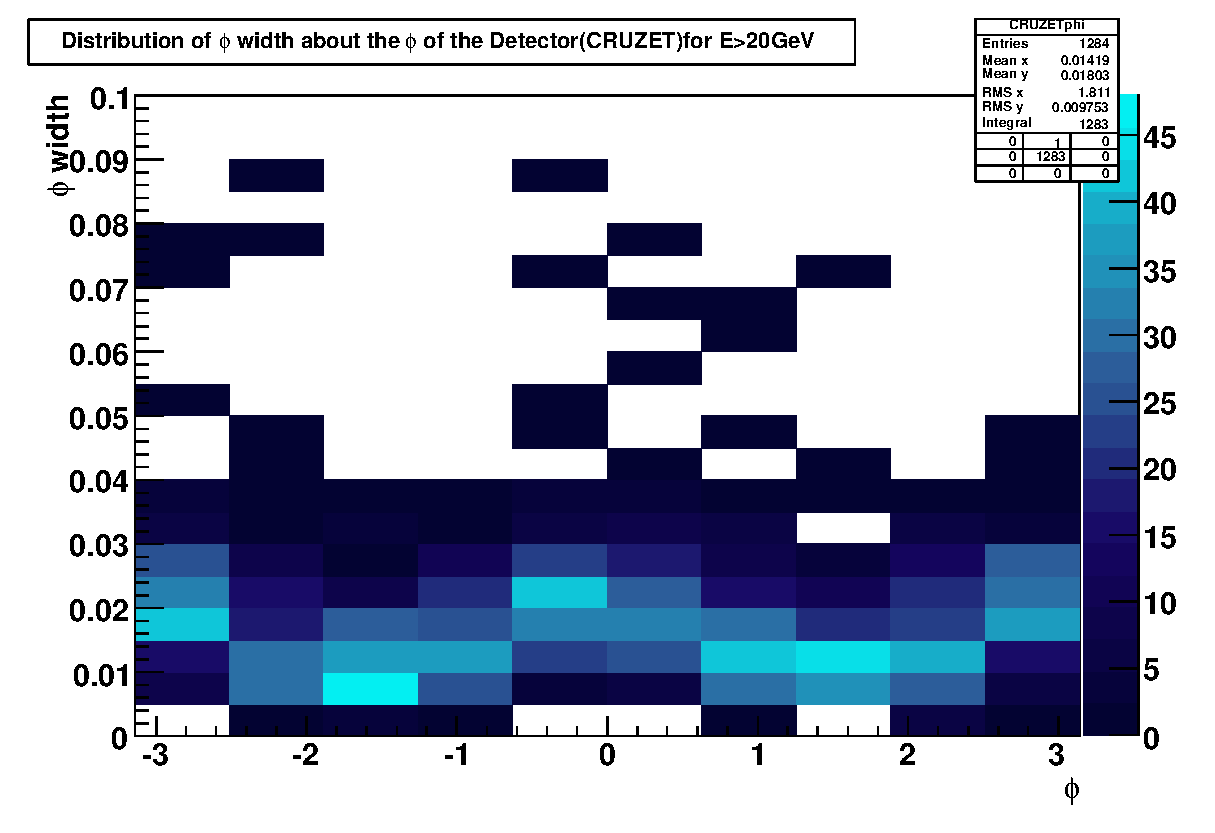
\includegraphics{CosmicPlots/CRUZET.eps}}
    \caption{The energy weighted width in $\phi$ as a function of detector $\phi$ for electromagnetic objects found in
CRUZET events.}
    \label{fig:CRUZETPhiWidPhi}
  \end{center}
\end{figure}

\subsubsection{ECAL - Muon Correlations}


\section{Summary}

\begin{thebibliography}{9}
\bibitem{NancyConv}  CMSNote XXXX


\end{thebibliography}
 
%------------------------------------------------------------------------------
\pagebreak
\appendix
\section{Photon Energy Scale}

\section{Photon Software Organization and Use}
The software for the reconstruction and identification of photons is logically
split into two parts.  The first, is the CVS package RecoEgamma/EgammaPhotonProducers.  For each ECAL 
supercluster in the barrel or endcap which meets the preselection requirements, a reco::Photon object 
is created.  At the time of this writing, the preselection requirements are simply that the 
supercluster must be at least 10~GeV in $E_T$, though additional switches for cuts on $HadOverEM$ 
and isolation are included for future use.  The second part of the software infrastructure is the
CVS package RecoEgamma/PhotonIdentification.  For every reco::Photon object that is created, a corresponding
reco::PhotonID object is created, and an association made and stored in the Event.
The purpose of the reco::Photon object is to organize most of the reconstruction level quantities associated
with the photon (the supercluster, the presence or absence of conversion tracks, the calculated photon 
position, etc.).  The purpose of the ``helper'' object reco::PhotonID is to provide additional information
in order to allow users to select reconstructed photon objects that satisfy at least the criteria set
forth in this note.  The reco::PhotonID object (stored in DataFormats/EgammaCandidates) contains information
on the isolation of the photon (calculated using the RecoEgamma/EgammaIsolationAlgos) as well as several
flags concerning the position of the photon with respect to both the barrel-endcap junction and the 
supermodule boundaries and fiducial locations in detector $\eta-\phi$.  Quality flags, defined for {\bf LooseEM}, {\bf LoosePhoton} and {\bf TightPhoton} are also set based on the criteria defined in the configuration file.

\section{Photon Identification at High Energies}

\end{document}
